\chapter{\Large Iteración II: “Información contextual y envió de alertas de seguridad”}
\label{iteracion2}
    Partiendo de la topología definida en la Figura \ref{fig:iter1_top_m_unc} de Iteración I, se procedió a verificar los requerimientos de prioridad media. Para ello se siguió con la misma metodología de prueba, que consistió en un escaneo de puertos desde una terminal dentro de la Dependencia 1 a un activo ubicado dentro del datacenter llamado Servidor 1.
    \begin{section}{Verificación de RF2: Recolección de información contextual}
    Con el objetivo de recibir y procesar información contextual de los activos que se ven afectados durante un incidente, fue necesario configurar el servidor Master de Security Onion, con otros servicios que permitieran recibir información diferente de la provista por los sensores. Esta información refleja el estado de los servicios en un servidor, su conexión a la red, parámetros de uso de hardware como el nivel de ocupación de disco, temperatura, uso de la memoria RAM, los logs referidos al procesamiento de las peticiones que recibe un servidor, etc. \par
     Una anomalía en los datos de esta información no es suficiente por sí misma para confirmar un ataque, pero es útil para indicar que algo puede estar ocurriendo. En el caso de un ataque confirmado, estos datos representan evidencia forense y sirven para enriquecer modelos de amenazas complejas. \par
     Se decidió enviar la información contextual disponible mediante Filebeat. Este es un servicio que permite enviar información a Logstash desde múltiples directorios. El proceso comienza cuando el servicio lee línea por línea los archivos de entrada y envía los logs de la misma manera a Logstash. Este los recibe en su puerto 5044 por defecto, posteriormente puede filtrarlos para separar los campos de los logs o bien almacenarlos sin filtrar. \par
     Al principio se envió los logs del estado de las aplicaciones de un servidor disponible en la organización, mediante Filebeat, a Logstash y sin un procesamiento posterior. Esto generó que ElastAlert no pudiera realizar una correlación al no identificar información clave, como la que se encuentra en los campos de puertos y direcciones IP de origen y destino, estampas de tiempo, tipo de peticiones, etc.\par
     Posteriormente se utilizó el plugin Grok para filtrar los logs que estaba recibiendo Logstash antes de almacenarlos, de manera que la detección basada en correlaciones fue posible.\par
      Como se observa en la Figura \ref{fig:figura_iter2_ataque}, se realizó el envío de logs del Servidor 1 (que se encuentra conectado al Switch 3) mediante Filebeat al nodo Master que se encuentra conectado al Switch 4. Estos logs contenían información de un servidor web Apache, incluyendo consultas realizadas, métodos y otros metadatos de interés. Esta información resultó útil para identificar un ataque de fuerza bruta de estilo “inyección SQL”, que fue simulado utilizando herramientas como “sqlmap”, desarrolladas en Python 3.5. Este tipo de ataque consiste en introducir, de manera iterativa, comandos SQL en un formulario web con el objetivo de lograr recabar información de las bases de datos del Servidor 1 (víctima), modificar e incluso eliminar dicha base de datos. El comando utilizado en sqlmap fue: 
      \textit{python sqlmap.py -u "http://IP\_VICTIMA/login/index.php?id=101" --batch} donde los flags significan:
      \begin{itemize}
          \item \textit{-u}: parámetro para especificar una URL.
          \item \textit{“http://IP\_victima/path/al/formulario?etc”} es el campo que contiene la dirección de un formulario en la página web víctima.
          \item \textit{--batch}: es un switch que sirve para elegir la opción por defecto en paginas donde hay múltiples parámetros. La consecuencia de elegir la opción por defecto es que ahorra tiempo al evitar una elección del usuario.
      \end{itemize}
    \begin{figure}[H]
        \centering
        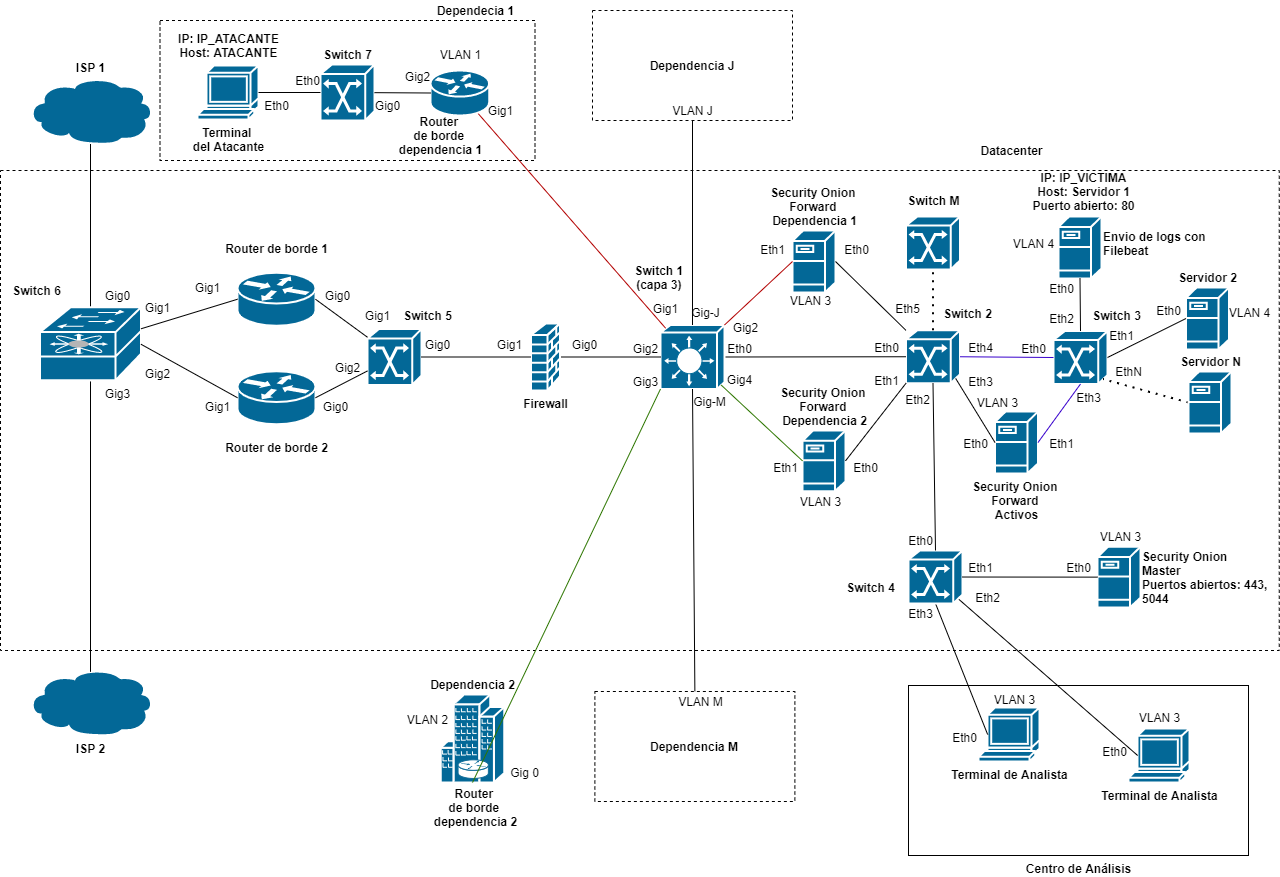
\includegraphics[width=1\textwidth]{./iteracion_2_imagenes/figura_iter2_ataque.png}
        \caption{Topología distribuida para la verificación de RF2, RF6 y RF4}
        \label{fig:figura_iter2_ataque}
    \end{figure}
    \FloatBarrier
    Como se mencionó anteriormente, en primer lugar los logs se almacenaron sin filtrar, lo que ocasionó que no fuese posible realizar algún tipo de correlación con los datos obtenidos. En la Figura \ref{fig:iter2_logs_crudos} se puede observar el almacenamiento de estos registros, con esto queda demostrado el cumplimiento del requerimiento funcional 2.
    \begin{figure}[H]
    \centering
        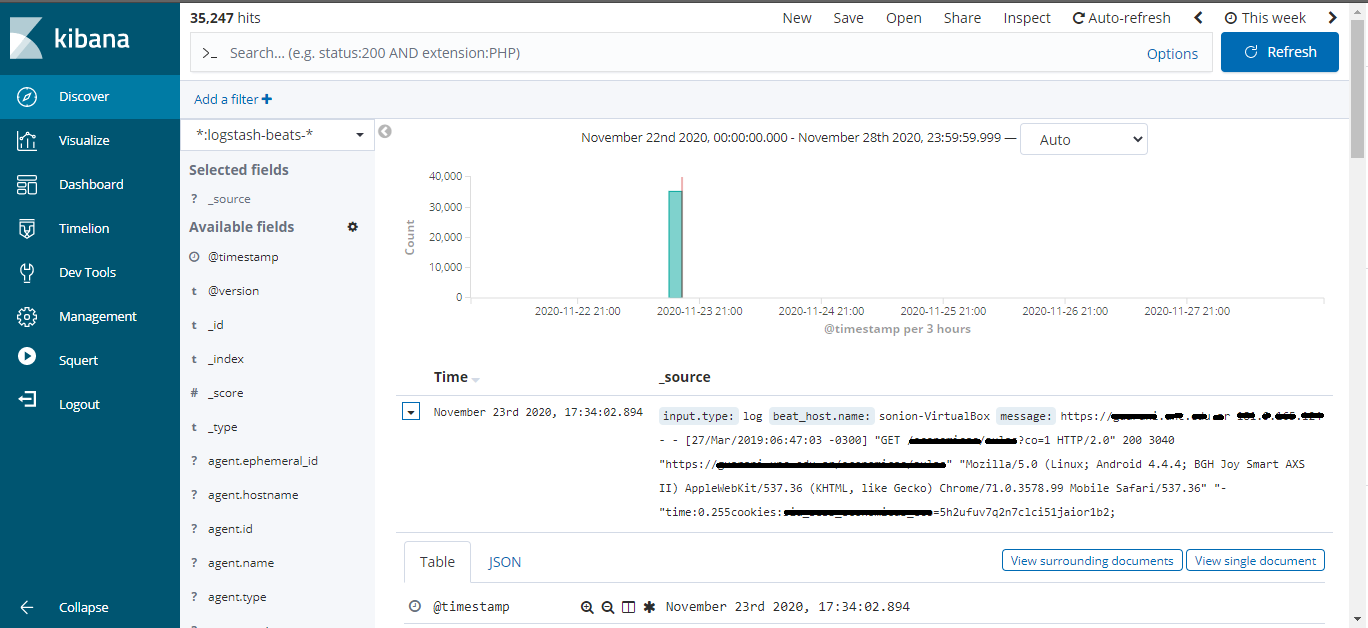
\includegraphics[width=1\textwidth]{./iteracion_2_imagenes/1_kibana_logs_1EDITADA.png}
        \caption{Almacenamiento de logs sin procesar}
        \label{fig:iter2_logs_crudos}
    \end{figure}
    Posteriormente se repitió la experiencia pero esta vez los logs que se recibían en Logstash eran procesados utilizando Grok. Este es un plugin de Logstash que permite filtrar datos sin ningún tipo de estructura y generar información estructurada capaz de ser consultada. \par
    En la Figura \ref{fig:figura_squert-sql} se pudo comprobar que el ataque de inyección SQL fue detectado en Squert.
    \begin{figure}[H]
    \centering
        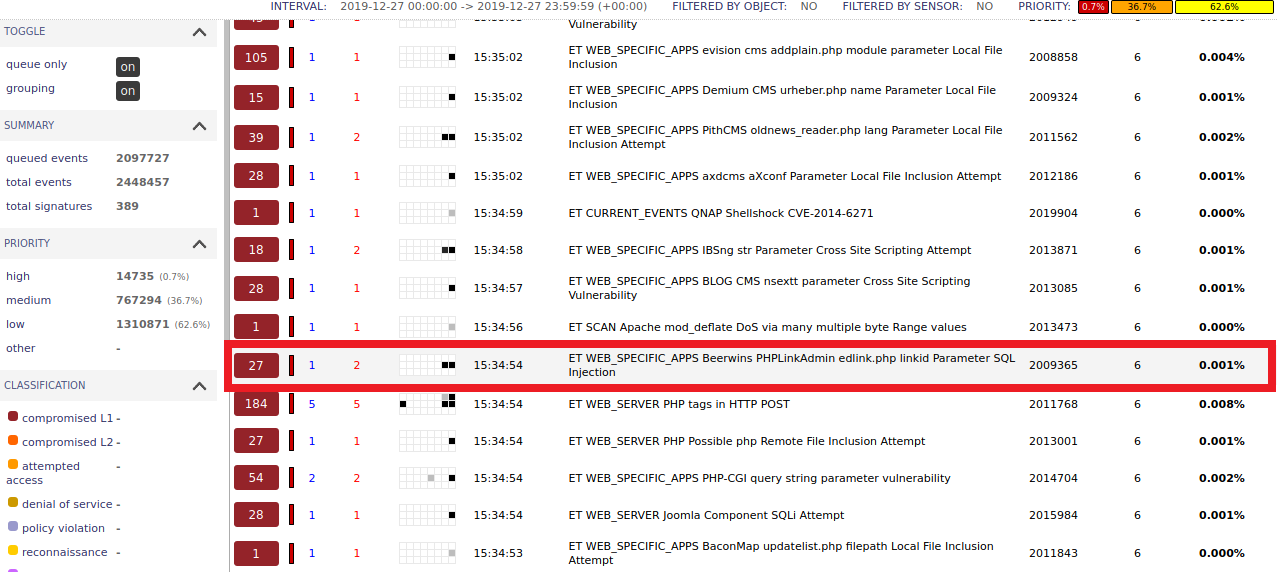
\includegraphics[width=0.7\textwidth]{./iteracion_2_imagenes/squert-sql-injection.png}
        \caption{Detección de un ataque de inyección SQL en el panel de Squert}
        \label{fig:figura_squert-sql}
    \end{figure}
    
    Los resultados en Kibana se ven en la Figura 6.3, donde se registraron las direcciones IP del Servidor 1 (víctima) y la del atacante. \par
    \begin{figure}[H]
    \centering
        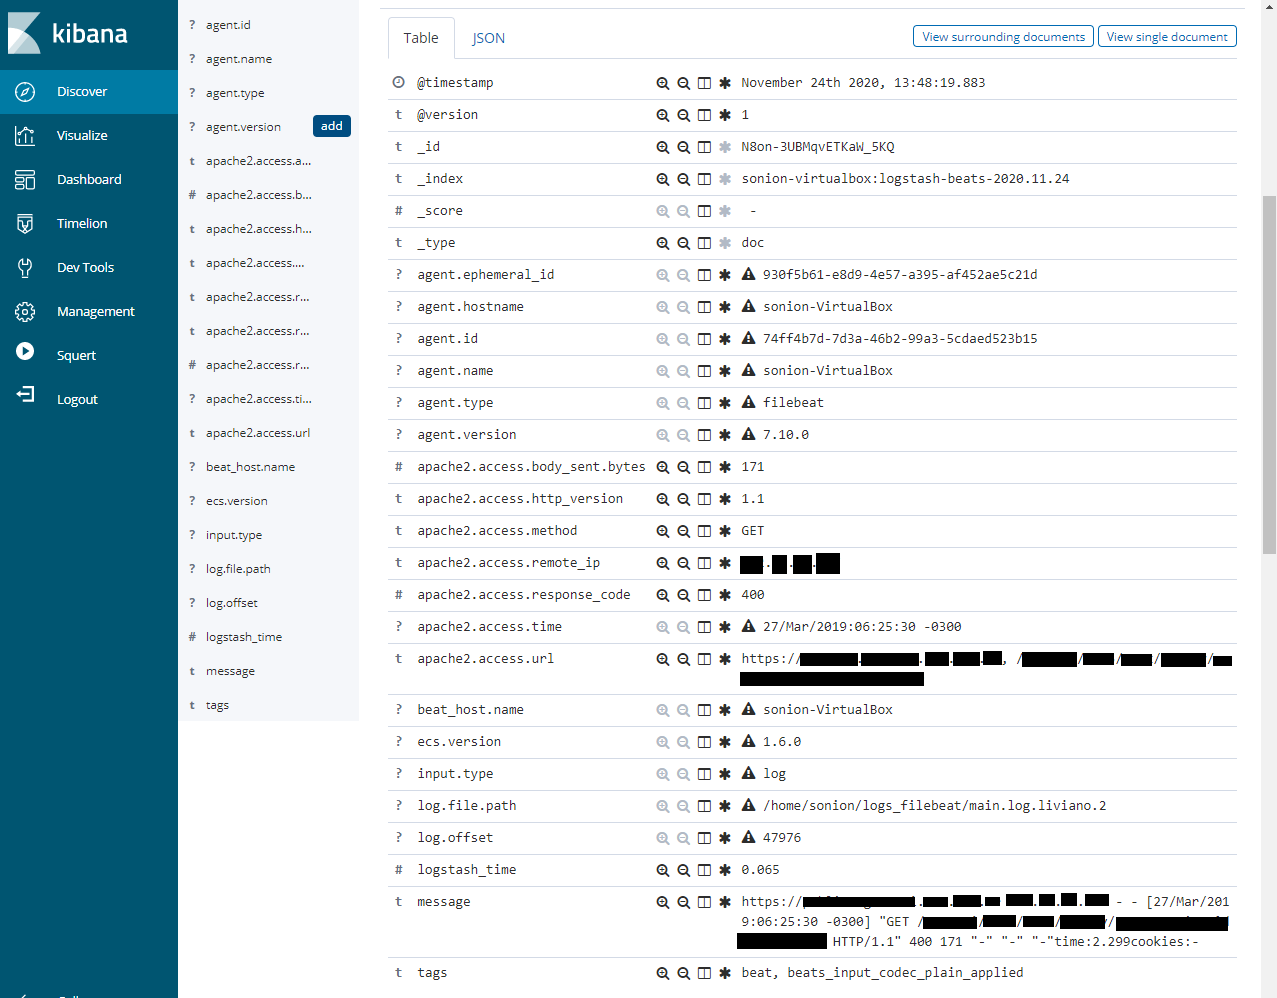
\includegraphics[width=1\textwidth]{./iteracion_2_imagenes/kibana_logs_parseados_2EDITADO.png}
        \caption{Almacenamiento de logs procesados por Logstash}
        \label{fig:iter2_logs_filtrados}
    \end{figure}
    
    Logstash posee varios filtros para todos los tipos de entradas que soporta. 
    Fue posible editar y administrar estos filtros utilizando archivos de configuración ubicados en la carpeta \textit{/etc/logstash/conf.d.available/}. Para este proyecto se eligió editar el filtro que procesa los datos provenientes de Filebeat, como se indicó anteriormente.\par
    Es importante mencionar que la información almacenada en Elasticsearch, es consultada constantemente por ElastAlert. Este último componente es el encargado de correlacionar los campos de los logs y enviar notificaciones.
    \end{section}
    \pagebreak
    
    \begin{section}{Verificación de RF6 y RF4: implementación de un sistema de correlación y envió de alertas de seguridad}
    El envío de alertas de seguridad y la notificación a los responsables de los activos que se ven afectados, fue realizado en este trabajo mediante ElastAlert. Este componente fue seleccionado ya que permite correlacionar la información presente en los campos de logs guardados en elasticsearch, así como enviar notificaciones cuando se produce la detección de incidentes. \par
    ElastAlert es un framework que detecta patrones en los datos consultados a Elasticsearch, como anomalías, picos, etc. Como se mencionó en la sección 4.5, basa su funcionamiento en dos componentes: reglas y alertas. \par
    Las alertas consisten en mensajes que permiten notificar a un usuario final o a otro sistema, sobre un evento de seguridad que ha ocurrido. Para esta prueba se decidió realizar nuevamente un escaneo de puertos desde el Atacante ubicado en la Dependencia 1 al Sevidor 1 víctima ubicado en el datacenter. Para esto se configuro a ElastAlert para que notifique por correo electrónico si este detectaba algún tipo de ataque de categoría “scan”.\par
     En la Figura \ref{fig:iter2_diagrama_envio_alertas} se observa un diagrama de secuencia del envío de una alerta.
    La secuencia comienza cuando los logs que llegan a Logstash son filtrados y enviados de forma estructurada (JSON) al puerto 9200 de Elastisearch. ElastAlert, por otro lado, realiza consultas periódicas a Elasticsearch. Cuando ElastAlert recibe una respuesta a su petición, procede a analizar los resultados en búsqueda de patrones que se puedan identificar en los logs recibidos. \par
    Independientemente de la coincidencia o no de algún patrón y la eventual notificación de alerta a los correspondientes responsables, ElastAlert vuelve a consultar a Elasticsearch por otros logs y procede a repetir el procedimiento descrito, mientras este activo como servicio.\par
    \begin{figure}[H]
    \centering
        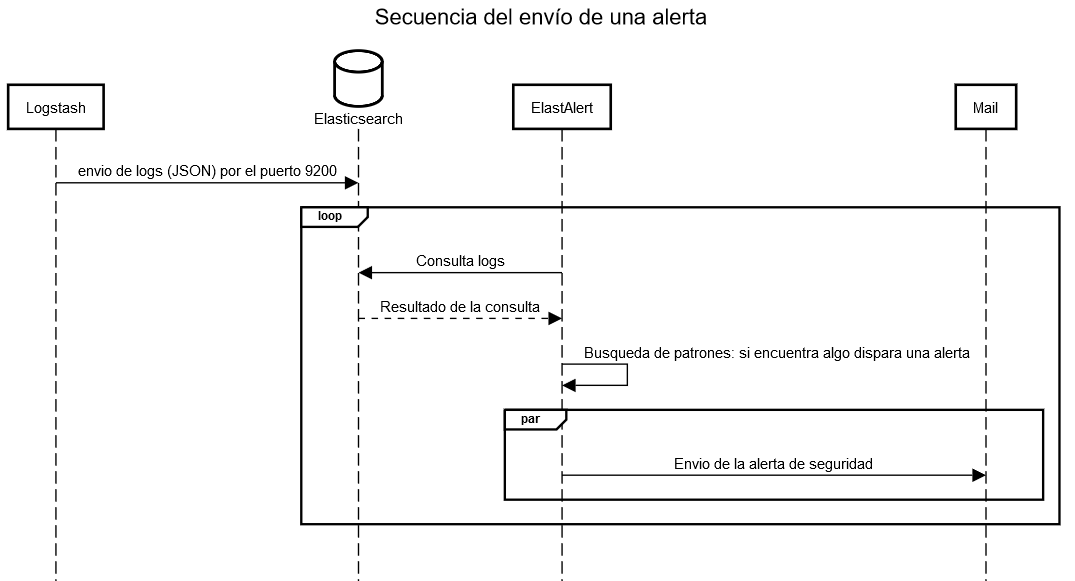
\includegraphics[width=1\textwidth]{./iteracion_2_imagenes/2-diagrama-de-secuencia-envio-alerta.png}
        \caption{Diagrama de secuencia del envío de una alerta}
        \label{fig:iter2_diagrama_envio_alertas}
    \end{figure}
    Los patrones a buscar están definidos en las reglas habilitadas de ElastAlert y si se produce una coincidencia, se procede a enviar una notificación por los medios especificados en las reglas. Como se mencionó anteriormente, para esta prueba el medio elegido fue el correo electrónico de la organización. En la Figura \ref{fig:iter2_notificacion_alertas} se observa el correo electrónico recibido cuando se disparó una alerta sobre un ataque de reconocimiento. Con esto damos por verificado los RF4 y RF6, dado que para que la notificación haya sido enviada, previamente se tuvo que ejecutar una correlación, como se describió anteriormente.\par
    \begin{figure}[H]
    \centering
        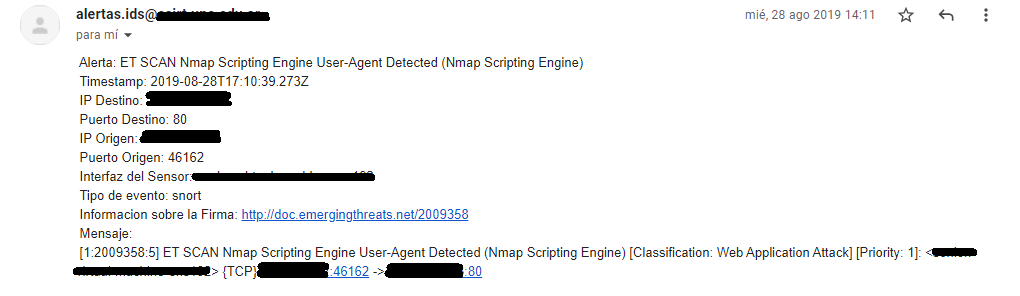
\includegraphics[width=1\textwidth]{./iteracion_2_imagenes/notificacion_alertas_1EDITADO.png}
        \caption{Notificación recibida debido a una alerta por reconocimiento de puertos}
        \label{fig:iter2_notificacion_alertas}
    \end{figure}
    
    \end{section}